

%----------------------------------------------------------------------------------------
%	PACKAGES AND OTHER DOCUMENT CONFIGURATIONS
%----------------------------------------------------------------------------------------

\documentclass[
11pt, % The default document font size, options: 10pt, 11pt, 12pt
%oneside, % Two side (alternating margins) for binding by default, uncomment to switch to one side
english, % ngerman for German
singlespacing, % Single line spacing, alternatives: onehalfspacing or doublespacing
%draft, % Uncomment to enable draft mode (no pictures, no links, overfull hboxes indicated)
%nolistspacing, % If the document is onehalfspacing or doublespacing, uncomment this to set spacing in lists to single
%liststotoc, % Uncomment to add the list of figures/tables/etc to the table of contents
%toctotoc, % Uncomment to add the main table of contents to the table of contents
%parskip, % Uncomment to add space between paragraphs
%nohyperref, % Uncomment to not load the hyperref package
headsepline, % Uncomment to get a line under the header
%chapterinoneline, % Uncomment to place the chapter title next to the number on one line
%consistentlayout, % Uncomment to change the layout of the declaration, abstract and acknowledgements pages to match the default layout
]{MastersDoctoralThesis} % The class file specifying the document structure

\usepackage[utf8]{inputenc} % Required for inputting international characters
\usepackage[T1]{fontenc} % Output font encoding for international characters

\usepackage{mathpazo} % Use the Palatino font by default

\usepackage[backend=bibtex,style=phys,natbib=true]{biblatex} % Use the bibtex backend with the authoryear citation style (which resembles APA)

\addbibresource{TFM.bib} % The filename of the bibliography

\usepackage[autostyle=true]{csquotes} % Required to generate language-dependent quotes in the bibliography

%----------------------------------------------------------------------------------------
%	CUSTOM PACKAGES
%----------------------------------------------------------------------------------------

\usepackage{bm}
\usepackage{physics}
\usepackage{amsmath}

%----------------------------------------------------------------------------------------
%	CUSTOM COMMANDS
%----------------------------------------------------------------------------------------

\newcommand{\D}[0]{\mathrm{d}}
\newcommand{\me}{\mathrm{e}}
\newcommand{\mi}{\mathrm{i}}
\newcommand{\oa}{\hat{a}}
\newcommand{\oad}{\hat{a}^\dagger}
\newcommand{\h}[1]{\hat{#1}}
\newcommand{\mr}[1]{\mathrm{#1}}
\newcommand{\pd}[2]{\frac{\partial{#1}}{\partial{#2}}}
\newcommand{\deriv}[2]{\frac{\D{#1}}{\D{#2}}}
\newcommand{\repr}{\,\dot{=}\,}
\newcommand\m[1]{\begin{pmatrix}#1\end{pmatrix}}

\newtheorem{theorem}{Theorem}

%----------------------------------------------------------------------------------------
%	MARGIN SETTINGS
%----------------------------------------------------------------------------------------

\geometry{
	paper=a4paper, % Change to letterpaper for US letter
	inner=2.5cm, % Inner margin
	outer=3.8cm, % Outer margin
	bindingoffset=.5cm, % Binding offset
	top=1.5cm, % Top margin
	bottom=1.5cm, % Bottom margin
	%showframe, % Uncomment to show how the type block is set on the page
}

%----------------------------------------------------------------------------------------
%	THESIS INFORMATION
%----------------------------------------------------------------------------------------

\thesistitle{Control of ribbon interaction in nanoporous graphene via pore functionalization} % Your thesis title, this is used in the title and abstract, print it elsewhere with \ttitle
\supervisor{Aran \textsc{Garcia-Lekue}\\ Daniel \textsc{Sánchez Portal}} % Your supervisor's name, this is used in the title page, print it elsewhere with \supname
%\supervisor{Daniel \textsc{Sánchez Portal}}
\examiner{} % Your examiner's name, this is not currently used anywhere in the template, print it elsewhere with \examname
\degree{Quantum Science and Technology} % Your degree name, this is used in the title page and abstract, print it elsewhere with \degreename
\author{Asier \textsc{Rodríguez Escalante}} % Your name, this is used in the title page and abstract, print it elsewhere with \authorname
\addresses{} % Your address, this is not currently used anywhere in the template, print it elsewhere with \addressname

\keywords{} % Keywords for your thesis, this is not currently used anywhere in the template, print it elsewhere with \keywordnames
\university{\href{https://www.ehu.eus/}{UPV-EHU}} % Your university's name and URL, this is used in the title page and abstract, print it elsewhere with \univname
\department{\href{http://department.university.com}{Department or School Name}} % Your department's name and URL, this is used in the title page and abstract, print it elsewhere with \deptname
\group{\href{http://researchgroup.university.com}{Research Group Name}} % Your research group's name and URL, this is used in the title page, print it elsewhere with \groupname
\faculty{\href{https://www.ehu.eus/en/web/zientzia-teknologia-fakultatea}{ZTF-FCT}} % Your faculty's name and URL, this is used in the title page and abstract, print it elsewhere with \facname

\AtBeginDocument{
\hypersetup{pdftitle=\ttitle} % Set the PDF's title to your title
\hypersetup{pdfauthor=\authorname} % Set the PDF's author to your name
\hypersetup{pdfkeywords=\keywordnames} % Set the PDF's keywords to your keywords
}

\begin{document}

\frontmatter % Use roman page numbering style (i, ii, iii, iv...) for the pre-content pages

\pagestyle{plain} % Default to the plain heading style until the thesis style is called for the body content

%----------------------------------------------------------------------------------------
%	TITLE PAGE
%----------------------------------------------------------------------------------------

\begin{titlepage}
\begin{center}

\vspace*{.06\textheight}
{\scshape\LARGE \univname\par}\vspace{1.5cm} % University name
\textsc{\Large Master's Thesis}\\[0.5cm] % Thesis type

\HRule \\[0.4cm] % Horizontal line
{\huge \bfseries \ttitle\par}\vspace{0.4cm} % Thesis title
\HRule \\[1.5cm] % Horizontal line
 
\begin{minipage}[t]{0.4\textwidth}
\begin{flushleft} \large
\emph{Author:}\\
\href{http://www.johnsmith.com}{\authorname} % Author name - remove the \href bracket to remove the link
\end{flushleft}
\end{minipage}
\begin{minipage}[t]{0.4\textwidth}
\begin{flushright} \large
\emph{Supervisors:} \\
\href{http://www.jamessmith.com}{\supname} % Supervisor name - remove the \href bracket to remove the link  
\end{flushright}
\end{minipage}\\[3cm]
 
\vfill

\large \textit{A thesis submitted in fulfillment of the requirements\\ for the  Master's degree in \degreename}\\[0.3cm] % University requirement text
%\textit{in the}\\[0.4cm]
%\groupname\\\deptname\\[2cm] % Research group name and department name
 
\vfill

{\large \today}\\[4cm] % Date
%\includegraphics{Logo} % University/department logo - uncomment to place it
 
\vfill
\end{center}
\end{titlepage}

%----------------------------------------------------------------------------------------
%	ABSTRACT PAGE
%----------------------------------------------------------------------------------------

\begin{abstract}
\addchaptertocentry{\abstractname} % Add the abstract to the table of contents
%The Thesis Abstract is written here (and usually kept to just this page). The page is kept centered vertically so can expand into the blank space above the title too\ldots
Lorem ipsum dolor sit amet, consectetur adipiscing elit, sed do eiusmod tempor incididunt ut labore et dolore magna aliqua. Ut enim ad minim veniam, quis nostrud exercitation ullamco laboris nisi ut aliquip ex ea commodo consequat. Duis aute irure dolor in reprehenderit in voluptate velit esse cillum dolore eu fugiat nulla pariatur. Excepteur sint occaecat cupidatat non proident, sunt in culpa qui officia deserunt mollit anim id est laborum.
\end{abstract}

%----------------------------------------------------------------------------------------
%	ACKNOWLEDGEMENTS
%----------------------------------------------------------------------------------------

\begin{acknowledgements}
\addchaptertocentry{\acknowledgementname} % Add the acknowledgements to the table of contents
%The acknowledgments and the people to thank go here, don't forget to include your project advisor\ldots
Lorem ipsum dolor sit amet, consectetur adipiscing elit, sed do eiusmod tempor incididunt ut labore et dolore magna aliqua. Ut enim ad minim veniam, quis nostrud exercitation ullamco laboris nisi ut aliquip ex ea commodo consequat. Duis aute irure dolor in reprehenderit in voluptate velit esse cillum dolore eu fugiat nulla pariatur. Excepteur sint occaecat cupidatat non proident, sunt in culpa qui officia deserunt mollit anim id est laborum.
\end{acknowledgements}

%----------------------------------------------------------------------------------------
%	LIST OF CONTENTS/FIGURES/TABLES PAGES
%----------------------------------------------------------------------------------------

\tableofcontents % Prints the main table of contents

\listoffigures % Prints the list of figures

\listoftables % Prints the list of tables

%----------------------------------------------------------------------------------------
%	ABBREVIATIONS
%----------------------------------------------------------------------------------------

\begin{abbreviations}{ll} % Include a list of abbreviations (a table of two columns)

\textbf{AGNR} & \textbf{A}rmchair-edged \textbf{G}raphene \textbf{N}ano\textbf{R}ibbon\\
\textbf{CB} & \textbf{C}onduction \textbf{B}and\\
\textbf{DFT} & \textbf{D}ensity \textbf{F}unctional \textbf{T}heory\\
\textbf{FFT} & \textbf{F}ast \textbf{F}ourier \textbf{T}ransform\\
\textbf{GGA} & \textbf{G}eneralized \textbf{G}radient \textbf{A}pproximation\\
\textbf{GNR} & \textbf{G}raphene \textbf{N}ano\textbf{R}ibbon\\
\textbf{HK} & \textbf{H}ohenberg-\textbf{K}ohn\\
\textbf{KB} & \textbf{K}leinman-\textbf{B}ylander\\
\textbf{KS} & \textbf{K}ohn-\textbf{S}ham\\
\textbf{LDA} & \textbf{L}ocal \textbf{D}ensity \textbf{A}pproximation\\
\textbf{NA} & \textbf{N}eutral \textbf{A}tom\\
\textbf{NAO} & \textbf{N}umerical \textbf{A}tomic \textbf{O}rbital\\
\textbf{NEGF} & \textbf{N}on-\textbf{E}quilibrium \textbf{G}reen's \textbf{F}unction\\
\textbf{NPG} & \textbf{N}ano\textbf{P}orous \textbf{G}raphene\\
\textbf{PAO} & \textbf{P}seudo \textbf{A}tomic \textbf{O}rbital\\
\textbf{PBE} & \textbf{P}erdew-\textbf{B}urke-\textbf{E}rnzerhof\\
\textbf{PW} & \textbf{P}lane \textbf{W}ave\\
\textbf{STM} & \textbf{S}canning \textbf{T}unneling \textbf{M}icroscope\\
\textbf{SCF} & \textbf{S}elf-\textbf{C}onsistent \textbf{F}ield\\
\textbf{VB} & \textbf{V}alence \textbf{B}and

\end{abbreviations}

%----------------------------------------------------------------------------------------
%	THESIS CONTENT - CHAPTERS
%----------------------------------------------------------------------------------------

\mainmatter % Begin numeric (1,2,3...) page numbering

\pagestyle{thesis} % Return the page headers back to the "thesis" style

% Include the chapters of the thesis as separate files from the Chapters folder
% Uncomment the lines as you write the chapters

% Chapter 1

\chapter{Introduction}

\label{ch1}

%----------------------------------------------------------------------------------------

% Define some commands to keep the formatting separated from the content 
\newcommand{\keyword}[1]{\textbf{#1}}
\newcommand{\tabhead}[1]{\textbf{#1}}
\newcommand{\code}[1]{\texttt{#1}}
\newcommand{\file}[1]{\texttt{\bfseries#1}}
\newcommand{\option}[1]{\texttt{\itshape#1}}

%----------------------------------------------------------------------------------------

Since Geim and Novoselov first isolated and charaterized of graphene\parencite{Geim2007} the study of its properties and applications has become an active and still growing field of research especially within condensed matter physics and materials science\parencite{Houtsma2021}. Graphene’s exceptional electronic properties, combined with its small volume, make it an ideal candidate for its use in electronic applications, yet its gapless, semimetallic nature prevents it from being used as a logic device with distinguishable ON and OFF states\parencite{Allen2010}. One way to do this is via electron confinement in one direction, in the form of graphene nanoribbons (GNRs).\\


**GNR to NPG: general reasons**\\
%After the emergence of bottom-up on-surface synthesis of organic covalent structures [1,2] Specifically designed organic molecules are deposited on metallic substrates where they self-assemble and, by increasing temperature, they bind through a surface-catalyzed reaction via specific functional groups, forming highly robust covalent nano-structures. [3] Over the years, a number of different types of carbon nanomaterials have been fabricated in this way, such as extended 2D covalent organic frameworks, [2,4,5] 1D and circular molecular oligomers, [3,6–8] 1D organic polymers, [9–11] and nanographenes. [12–15] Among all these, the so-called graphene nanoribbons [16,17] (GNRs), first reported via on-surface synthesis in 2010, [18] have received enormous attention as potential platforms for future carbon nanoelectronics. [19–22] This is partly because of their fully \(\pi\)-conjugated structure allowing for efficient electron transport, plus their confined dimensionality equipping them with an electronic band gap which is essential for logic-gate applications. In this direction, electron transport through GNRs has been measured multiple times in solid-state devices [23–26] and also on metallic surfaces using the tip of a scanning tunneling microscope (STM).\\


**Molecular switches: what for, applications?**\\
%Use of external stimuli (e.g. light, temperature, pH) to controllably induce molecular level structural and/or chemical changes can be exploited for using individual molecules like switches in electronic devices.1–3 Unlike the top-down fabrication of inorganic siliconbased transistors, molecular switches are synthesised via bottom-up chemical design. As such, there are many different examples of switchable molecular systems based on a wide range of chemistries.4 Since electric field (E-field) driven semiconductor-based switches are key components in electrical circuitry, in recent years extensive research efforts have been devoted to fabricating junctions of single-molecules or selfassembled monolayers whose conductance can be reversibly switched by means of external E-fields. Such E-field induced molecular switching can be achieved by means of changes in the redox state of electrochemically active molecules,5–7 molecular conformational rearrangements,


Relate molecular switches and sensing\\

**sensing: motivation and problems. NPG: array of sensors?\\
general properties of sensors (meng) + specific example (shekirev), not "accurate" enough(?) -> atomically precise array of sensors (talk about molecular switch sensors first)\\
%
** our proposal...**\\

\section{Thesis outline}

In chapter 2 we carefully describe the methods used for calculations in this thesis, namely density functional theory (DFT) through the program SIESTA, and the \textsc{sisl} Python package. Chapter 3 is a review of the state of the art regarding NPG structures and transport calculations within them, and we reproduce some results found in the literature. In chapter 4 our main results and calculations are presented, and chapter 5 summarizes our work and makes the concluding statements, as well as a discussion regarding future work.



% Chapter 1

\chapter{Theoretical and computational tools} % Main chapter title
% Theory and programs?

\label{Chapter1} % For referencing the chapter elsewhere, use \ref{Chapter1} 

%----------------------------------------------------------------------------------------

% Define some commands to keep the formatting separated from the content 
\newcommand{\keyword}[1]{\textbf{#1}}
\newcommand{\tabhead}[1]{\textbf{#1}}
\newcommand{\code}[1]{\texttt{#1}}
\newcommand{\file}[1]{\texttt{\bfseries#1}}
\newcommand{\option}[1]{\texttt{\itshape#1}}

%----------------------------------------------------------------------------------------
\section{Density Functional Theory}

Density-functional theory (DFT) is an approach to study the electronic structure of many-body problems, which allows the computational treatment large and complex systems. In fact, one of the reasons why DFT has become an essential tool in many areas of physics including condensed-matter theory is the increasing availability and power of computational processing. DFT is mainly based on the fact that any property of a system of many interacting particles can be viewed as a functional of the ground state
density [**martin]. The famous paper by Hohenberg and Kohn in 1964 [** in martin] laid the groundwork of modern DFT, while the formulation presented in a 1965 paper by Kohn and Sham [** in martin] has prevailed as one of the most useful approaches up to this day. In the following subsections we will present the basics of this method, and then review a specific implementation, namely SIESTA, which will be used throughout this work.


\subsection{Basics of DFT}
The goal is to solve the many-body problem through Schrödinger's equation.

\subsection{SIESTA}
summary: In this method the effect of
the core electrons is described by soft norm-conserving
pseudopotentials and the electronic structure of the valence
electrons is expanded in a basis set of numerical atomic orbitals with finite range
%----------------------------------------------------------------------------------------

%\section{Transport through NEGF}
%
%In this section the theory of nonequilibrium Green's functions (NEGF) will be presented, as the underlying theory of various programs that will be used (\textsc{TranSIESTA} *** and \textsc{TBrans}***) to study transport properties of the desired materials. Knowledge of (first- and second-quantized) quantum mechanics  will be assumed, and the starting point will be an equilibrium state, which will lay the foundations and the basic properties of Green's functions. We will then delve into NEGF through the Keldysh formalism, and afterwards explore a simple and conceptually useful reformulation of this theory by S. Datta \textit{et al}***. Finally, we will overview the implementation in \textsc{TranSIESTA}.
%
%
%\subsection{Equilibrium Green's functions}
%
%
%\subsection{Keldysh formalism}
%\subsection{TranSIESTA and TBtrans}
%\subsection{sisl}


 
% Chapter 3

\chapter{Study of nanoporous graphene}

\label{ch3}

\section{Plain NPG}
% general info (synthesis, properties)
% bands
% application

%----------------------------------------------------------------------------------------

\section{Double-pore NPG}
% general info (synthesis, 7-13, different configurations
% \subsection{Ribbon crosstalk}

%----------------------------------------------------------------------------------------

\section{Functionalized nanoporous graphene}
% Hopes
% Properties (whichever we get to)


% Chapter 4

\chapter{Results}

\label{ch4}

In this section, we will perform DFT calculations with SIESTA with the intent to investigate functionalization in \textit{para}-\textit{para} NPG. Firstly, we will look into basic PP-NPG and its properties. Secondly, some calculations will be performed concerning individual dinitro-biphenyl molecules, which represent the bridges of the PP-NPG after functionalization with nitro groups. Finally, using the knowledge we acquired from the previous calculations, we explore the nitro-functionalized PP-NPG and the properties that will affect electron transport in this material.

\section{\textit{Para-para} NPG}
\textit{Para-para} connections in NPG present an special property, namely, the fact that both phenyls are able to be rotated through a central axis. It is known that phenyl-ring chains have trasport properties that depend on the torsional angle between the rings\parencite{Viljas2008}, which raises the question of what the effect of the torsional angle of the phenyl rings with respect to the 7-13-AGNR ribbon and with respect to one another might be, in terms of the inter-ribbon cross-talk. For this purpose, we study the electronic structure of PP-NPG.

Firstly, we obtained the relaxed structure up to a 0.01eV/\(\AA\) tolerance using the same parameters as for the basic NPG in section \ref{ele-npg}.
Equivalent and nonequivalent ribbons
% Pore orientation
%\subsection{Cross-talk}
Meaning\\
A measure of crosstalk \(\Delta E\) at \(\Gamma\)\\

\begin{figure}[h!]
	\centering
	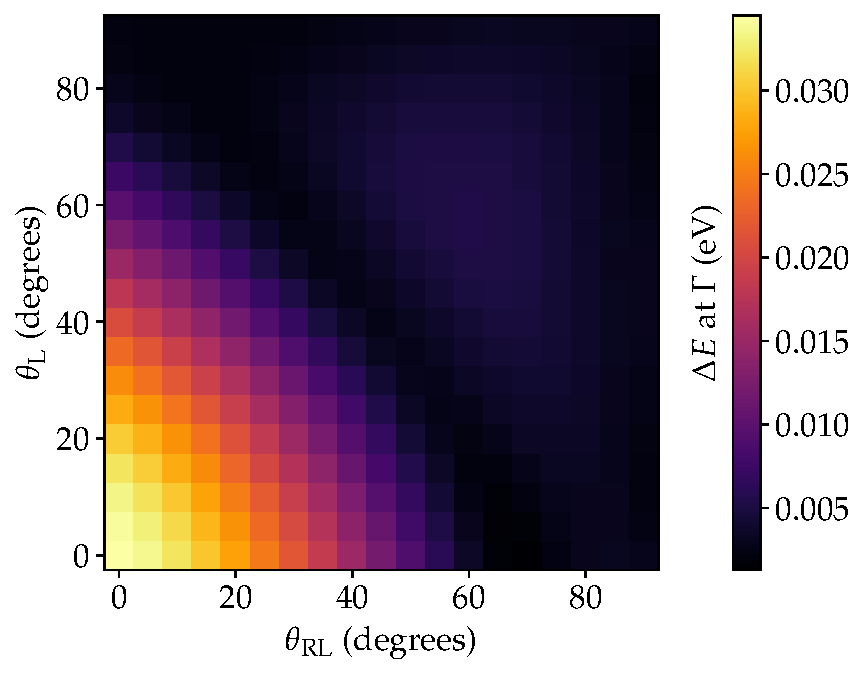
\includegraphics[width=0.7\linewidth]{Figures/2dmap}
	\decoRule
	\caption{2-dimensional plot of the band splitting of CB and CB+1 at the \(\Gamma\) point of PP-NPG.}
	\label{fig:2dmap}
\end{figure}


2D map. Decrease etc., 75\(^{\circ}\), from 3NN interaction in a TB picture?


\section{Dinitro-biphenyl molecule}
Properties (structure, (P)DOS...)\\
Molecular orbitals\\
Effect of the electric field (angle vs. \(\abs{\bm E}\), energy vs. angle...)

%----------------------------------------------------------------------------------------

\section{Dinitro-PP-NPG}
Resonance. Crosstalk

 
% Chapter 3

\chapter{Conclusions and outlook}

\label{ch5}

\section{Conclusions}


%----------------------------------------------------------------------------------------

\section{Outlook}
% general info (synthesis, 7-13, different configurations
% \subsection{Ribbon crosstalk}



%----------------------------------------------------------------------------------------
%	THESIS CONTENT - APPENDICES
%----------------------------------------------------------------------------------------

\appendix % Cue to tell LaTeX that the following "chapters" are Appendices

% Include the appendices of the thesis as separate files from the Appendices folder
% Uncomment the lines as you write the Appendices

%% Appendix A

\chapter{Frequently Asked Questions} % Main appendix title

\label{AppendixA} % For referencing this appendix elsewhere, use \ref{AppendixA}

\section{How do I change the colors of links?}

The color of links can be changed to your liking using:

{\small\verb!\hypersetup{urlcolor=red}!}, or

{\small\verb!\hypersetup{citecolor=green}!}, or

{\small\verb!\hypersetup{allcolor=blue}!}.

\noindent If you want to completely hide the links, you can use:

{\small\verb!\hypersetup{allcolors=.}!}, or even better: 

{\small\verb!\hypersetup{hidelinks}!}.

\noindent If you want to have obvious links in the PDF but not the printed text, use:

{\small\verb!\hypersetup{colorlinks=false}!}.

%\include{Appendices/AppendixB}
%\include{Appendices/AppendixC}

%----------------------------------------------------------------------------------------
%	BIBLIOGRAPHY
%----------------------------------------------------------------------------------------

\printbibliography[heading=bibintoc]

%----------------------------------------------------------------------------------------

\end{document}  
